% Векторизация перемножения матриц специального вида.
\subsection{Потери производительности из-за неполного \\ использования элементов векторных регистров}\label{sec:text_4_spec_matr}

В предыдущем разделе рассматривались матрицы размера $8 \times 8$ и $16 \times 16$, работа с которыми удобна в плане векторизации, так как в один векторных регистр помещается ровно 8 значений формата double или 16 значений формата float.
Однако, при работе с другими размерностями неизбежно возникает проблема неполного использования элементов векторных регистров, что приводит к падению производительности.
Рассмотрим эту проблему на конкретном примере.

При проведении вычислений с помощью метода RANS/ILES\label{abbr:rans2}\label{abbr:iles2} расчетные параметры компонуются внутри матриц размером $5 \times 5$, при этом данные матрицы являются подматрицами матриц размера $8 \times 8$ (это делается из соображений выровненности расположения в памяти).
Будем рассматривать операцию перемножения таких матриц и возможные пути повышения производительности этой операции \cite{Bendersky2018VecMat1}. 

\begin{figure}[ht]
\centering
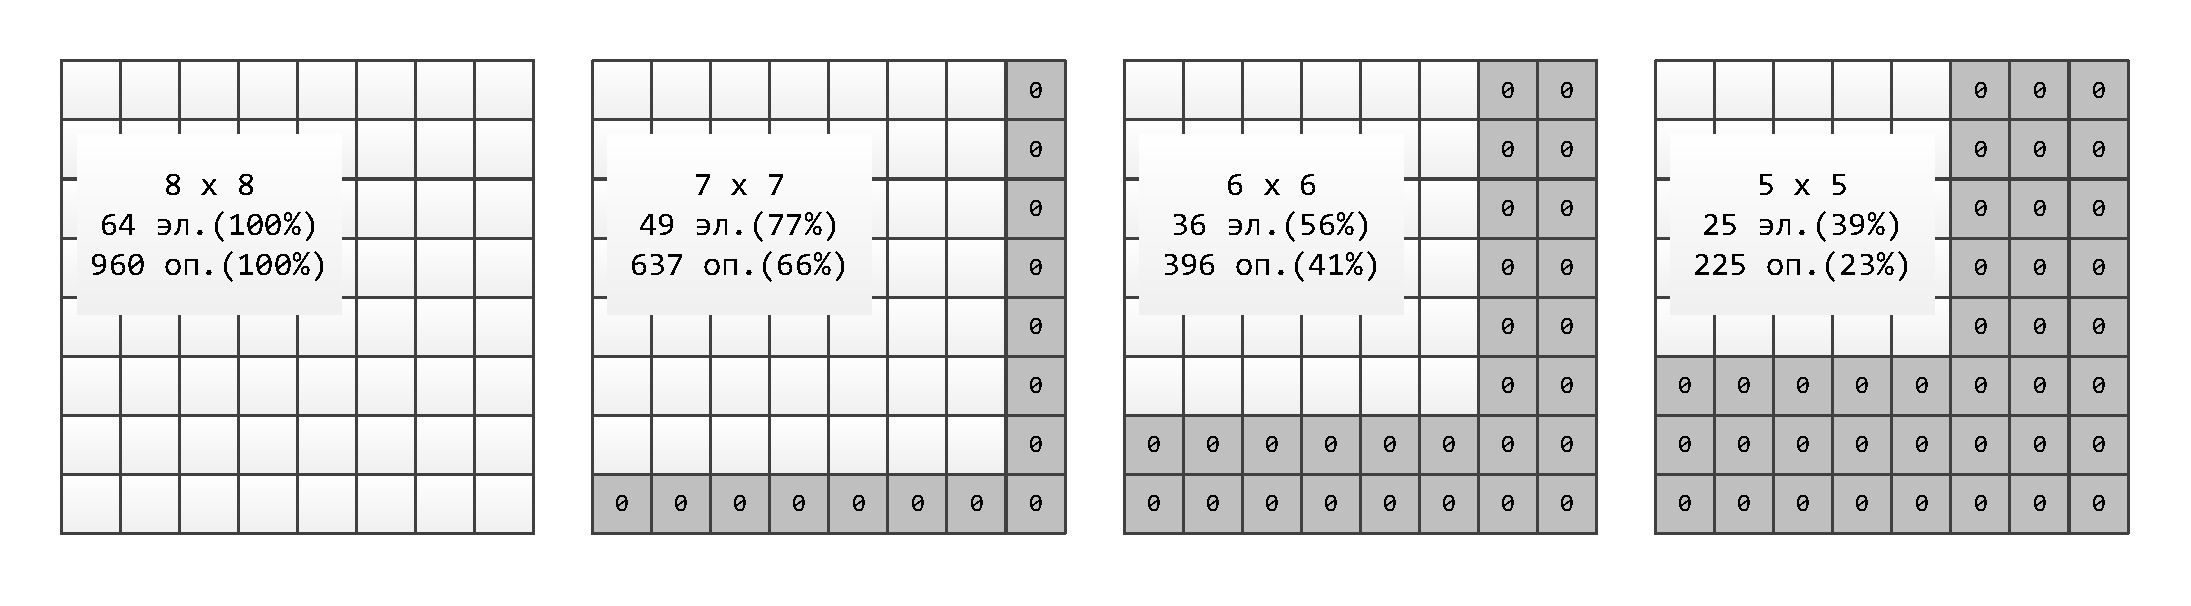
\includegraphics[width=1.00\textwidth]{./pics/text_4_spec_matr/matrices.pdf}
\singlespacing
\captionstyle{center}\caption{Иллюстрация матриц размера $8 \times 8$, $7 \times 7$, $6 \times 6$, $5 \times 5$, представленных как подматрицы матрицы $8 \times 8$.}
\label{fig:text_4_spec_matr_matrices}
\end{figure}

Основная идея векторизации перемножения матриц размера $8 \times 8$ и $16 \times 16$, рассмотренной в предыдущем разделе, заключалась в том, что вначале выполнялось поэлементное перемножение строк первой матрицы на столбцов второй матрицы, а затем параллельно вычислялась сумма элементов соответствующих векторов.
В случае матриц $16 \times 16$ параллельно вычислялась сумма элементов 16 векторов, в случае матриц $8 \times 8$ параллельно вычислялась сумма элементов половинок 8 векторов.
Достигалось это последовательным применением шаблонных связок, состоящих из операций perm, add и blend (см. листинги~\ref{lst:text_4_small_matr_swiz_macro} и \ref{lst:text_4_small_matr_matmat_opt}).

Эта реализация обладает существенными недостатками.
Во-первых, в коде присутствуют медленные инструкции gather/scatter, читающие из памяти элементы данных с произвольными смещениями, которые выполняются существенно медленнее чтения из памяти последовательных данных.
Во-вторых, выполнение сначала поэлементного перемножения векторов, а затем параллельное нахождение сумм их элементов (в данном случае рассчитываются суммы элементов половинок векторов), делают невозможным использование эффективных комбинированных инструкций fmadd.
Рассмотрим пути по устранению перечисленных недостатков.

\subsubsection{Оптимизация перемножения матриц с целью использования комбинированных операций}

Запишем в явном виде значения элементов $i$-й строки результирующей матрицы:
\begin{equation}
	\left\{
		\begin{aligned}
			& r_{i0} = a_{i0}b_{00} + a_{i1}b_{10} + \cdots + a_{i7}b_{70} \\
			& \cdots \\
			& r_{i7} = a_{i0}b_{07} + a_{i1}b_{17} + \cdots + a_{i7}b_{77}
		\end{aligned}
	\right.
\end{equation}

или в векторном виде
\begin{equation}\label{eqn:text_4_spec_matr_ri}
	\overline{r}_i = a_{i0}\overline{b}_0 + a_{i1}\overline{b}_1 + \cdots + a_{i7}\overline{b}_7
\end{equation}

Аналогичные выражения можно записать для строки с номером $i + 1$:
\begin{equation}
	\left\{
		\begin{aligned}
			& r_{i + 1,0} = a_{i + 1,0}b_{00} + a_{i + 1,1}b_{10} + \cdots + a_{i + 1,7}b_{70} \\
			& \cdots \\
			& r_{i + 1,7} = a_{i + 1,0}b_{07} + a_{i + 1,1}b_{17} + \cdots + a_{i + 1,7}b_{77}
		\end{aligned}
	\right.
\end{equation}

или в векторном виде
\begin{equation}\label{eqn:text_4_spec_matr_rip1}
	\overline{r}_{i + 1} = a_{i + 1,0}\overline{b}_0 + a_{i + 1,1}\overline{b}_1 + \cdots + a_{i + 1,7}\overline{b}_7
\end{equation}

Учитывая то, что zmm регистры содержат по 16 элементов типа float, то целесообразно объединить \eqref{eqn:text_4_spec_matr_ri} и \eqref{eqn:text_4_spec_matr_rip1} в одну формулу, записанную в векторном виде следующим образом:
\begin{equation}\label{eqn:text_4_spec_matr_riip1}
	\overline{r}|_{i + 1}^i
	=
	\sum_{j = 0}^{7} \left(  \overline{a}|_{i + 1,j}^{ij} \circ \overline{b}|_j^j \right)
\end{equation}

где $\overline{r}|_{i + 1}^i$ обозначает комбинированный вектор состоящий из векторов $\overline{r}_i$ и $\overline{r}_{i + 1}$, $\overline{b}|_j^j$ обозначает комбинированный вектор состоящий из двух копий вектора $\overline{b}_j$, а выражение $\overline{a}|_{i + 1,j}^{ij}$ обозначает вектор, первые 8 элементов которого равны $a_{ij}$, а остальные 8 элементов -- $a_{i + 1,j}$ ($\circ$ -- произведение Адамара\label{term:hadamar_mul}, или поэлементное произведение векторов).
Заметим, что получающийся по формуле \eqref{eqn:text_4_spec_matr_riip1} комбинированный вектор $\overline{r}|_{i + 1}^i$ расположен в памяти последовательно, и записывать его в память можно с помощью интринсика \texttt{\_mm512\_store\_ps}.
При этом предполагаем, что значение $i$ четно, то есть вектор $\overline{r}|_{i + 1}^i$ выровнен в памяти должным образом.
Другие комбинированные векторы в \eqref{eqn:text_4_spec_matr_riip1} получаются с помощью инструкции perm (интринсик \texttt{\_mm512\_permutexvar\_ps}), примененной к соответствующим загруженным соседним строкам матриц $a$ и $b$.
Таким образом, при реализации \eqref{eqn:text_4_spec_matr_riip1} не требуется использование медленных инструкций gather/scatter, так как столбцы матриц не читаются и не записываются (работа ведется только со строками).
После того, как векторы $\overline{a}|_{i + 1,j}^{ij}$ и $\overline{b}|_j^j$ сформированы, нужно выполнить их попарное поэлементное перемножение, после чего сложить в один вектор (8 операций поэлементного умножения, 7 операций сложения).
Эти действия можно выполнить, используя комбинированные операции fmadd.

\begin{figure}[ht]
\centering
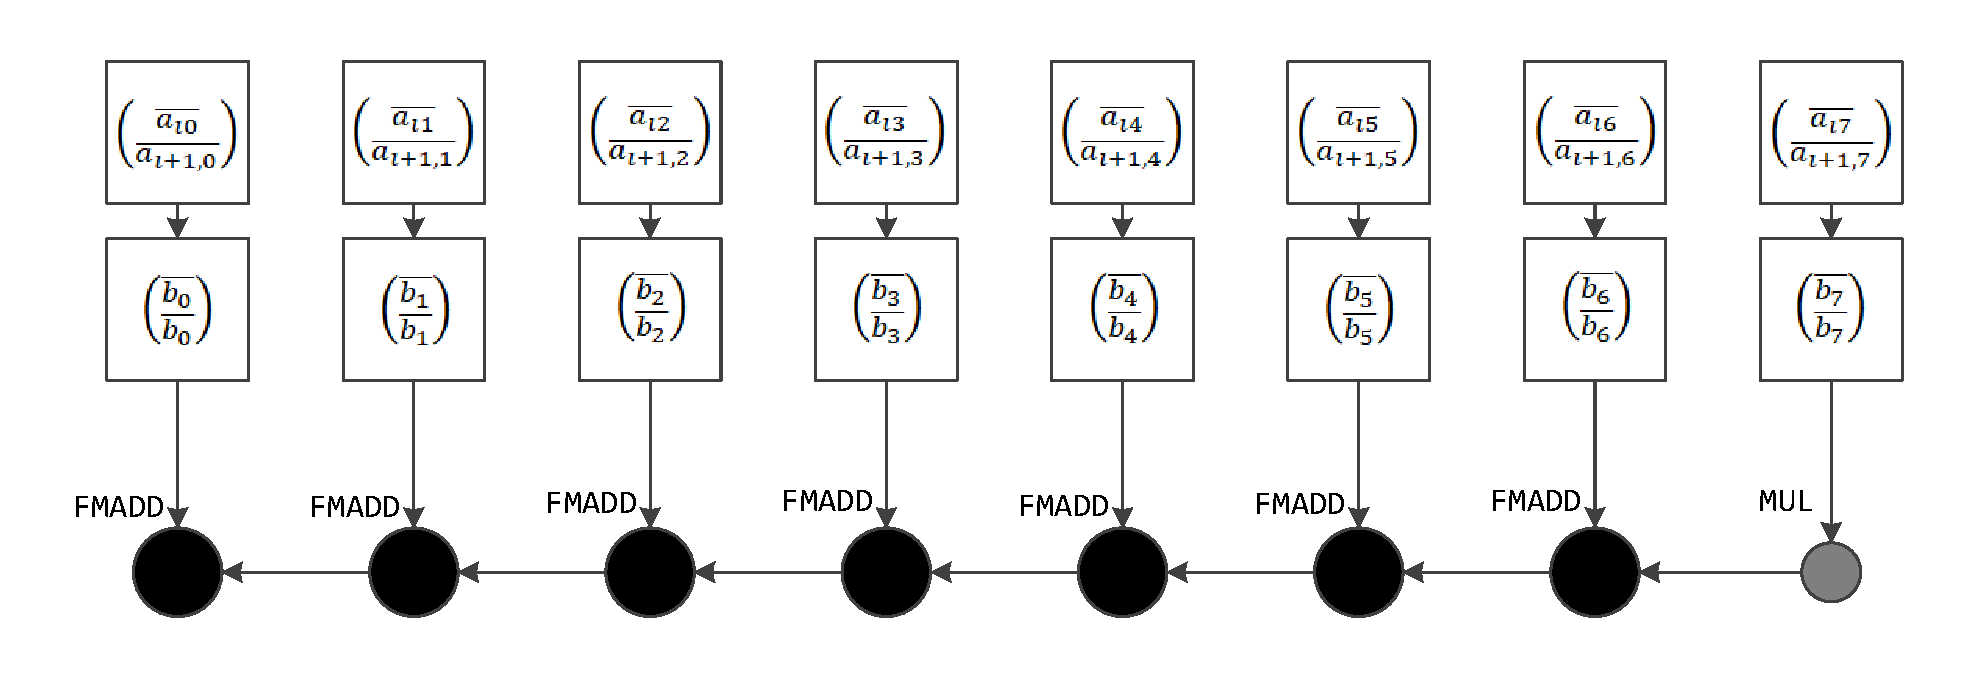
\includegraphics[width=1.00\textwidth]{./pics/text_4_spec_matr/fmadd.pdf}
\singlespacing
\captionstyle{center}\caption{Схема вычисления двух соседних строк результирующей матрицы путем последовательного сложения попарно перемноженных векторов.}
\label{fig:text_4_spec_matr_fmadd}
\end{figure}

Для вычисления значения $\overline{r}|_{i + 1}^i$ потребуется 8 векторных операций (1 операция mul и 7 операций fmadd) (см. рис.~\ref{fig:text_4_spec_matr_fmadd}).
На этом рисунке для удобства представлена схема последовательного сложения перемноженных векторов. Возможен также другой вариант, реализующий вычисление $\overline{r}|_{i + 1}^i$ с помощью балансировки дерева потока данных.
Такой вариант потребует 4 операций mul, 4 операций fmadd и 3 операций add.
В рассматриваемом контексте вычислений длина критической цепочки не влияет на время работы кода, поэтому мы оставляем вариант с минимальным количеством инструкций (меньше 8 инструкций задействовать невозможно, так как нужно выполнить по крайней мере 8 операций умножения).

\subsubsection{Посчет количества избыточных операций при перемножении матриц}

Приведем функцию перемножения двух матриц размера $8 \times 8$, с помощью использования комбинированных операций.
Для реализации выполним полную загрузку обеих матриц $a$ и $b$.
На это потребуется 8 операций обращения в память, так как за одну операцию загружаются две соседние строки матрицы.
Далее требуется сформировать 8 векторов вида $\overline{b}|_j^j$, для чего потребуется еще 8 операций perm (для каждой пары загруженных строк матрицы $b$ нужно выполнить дублирование первой строки и дублирование второй строки).

После подготовки всех необходимых данных выполняется вычисление значений результирующей матрицы.
Приведенный ниже блок операций (макрос \texttt{BLOCK}) осуществляет вычисление двух соседних строк результирующей матрицы.
Реализация блока состоит из 8 операций perm, 1 операции mul и 7 операций fmadd, кроме того выполняется одна операция записи в память.
Всего выполняется четыре таких блока, что в сумме и с учетом операций подготовки данных приводит к следующему итогу: 8 простых операций чтения из памяти, 40 операций perm, 4 операции mul, 28 операций fmadd, 4 простые операции записи в память.
Итоговый код (без отображения некоторых повторяющихся участков) приведен на листинге~\ref{lst:text_4_spec_matr_mul8x8_opt}.

\begin{lstlisting}[caption={Векторизованная версия перемножения матриц $8 \times 8$.},label={lst:text_4_spec_matr_mul8x8_opt}]
void mul_8x8_opt(float* __restrict a, float* __b, float* __restrict r)
{
    ...
    ind_df = _mm512_set_epi32(7,6,5,4,3,2,1,0,7,6,5,4,3,2,1,0);
    ind_ds = _mm512_set_epi32(15,14,13,12,11,10,9,8,
                              15,14,13,12,11,10,9,8);
    ...
    b0 = LD(&b[0]);
    b1 = _mm512_permutexvar_ps(ind_ds, b0);
    b0 = _mm512_permutexvar_ps(ind_df, b0);
    ...
    b6 = LD(&b[6 * V8]);
    b7 = _mm512_permutexvar_ps(ind_ds, b6);
    b6 = _mm512_permutexvar_ps(ind_df, b6);

    a0 = LD(&a[0]);
    ...
    a6 = LD(&a[6 * V8]);

    ind_0 = _mm512_set_epi32(8,8,8,8,8,8,8,8,0,0,0,0,0,0,0,0);
    ...
    ind_7 = _mm512_set_epi32(15,15,15,15,15,15,15,15,
                             7,7,7,7,7,7,7,7);

#define BLOCK(N, A)                           \
    ST(&r[N * V8],                            \
      FMADD(PERMXV(ind_0, A), b0,             \
        FMADD(PERMXV(ind_1, A), b1,           \
          FMADD(PERMXV(ind_2, A), b2,         \
            FMADD(PERMXV(ind_3, A), b3,       \
              FMADD(PERMXV(ind_4, A), b4,     \
                FMADD(PERMXV(ind_5, A), b5,   \
                  FMADD(PERMXV(ind_6, A), b6, \
                    MUL(PERMXV(ind_7, A), b7)))))))));

    BLOCK(0, a0);
    BLOCK(2, a2);
    BLOCK(4, a4);
    BLOCK(6, a6);
}
\end{lstlisting}

Полные тексты приведенного в разделе программного кода доступны в \cite{iparGithub}.

Заметим, что 28 векторных операций fmadd и 4 векторные операции mul соответствуют $(28 \times 2 + 4) \times 16 = 960$ скалярным операциям, что в точности совпадает с количеством скалярных операций, требуемых для выполнения перемножения двух матриц размера $8 \times 8$.
Таким образом, в предложенной реализации нет лишних арифметических операций, и результат каждой выполненной операции влияет на конечный результат.

При реализации перемножения матриц размера $7 \times 7$, $6 \times 6$, $5 \times 5$ удаляются заведомо лишние векторные операции (например, умножение на вектор, все элементы которого равны нулю), однако все равно остаются элементы векторов, обработка которых избыточна, что приводит к снижению эффективности векторизации в этих случаях.
Приведем таблицу с точным подсчетом количества скалярных операций для невекторизованных функций и количества векторных операций для их векторизованных аналогов (см. таблицу~\ref{tbl:text_4_spec_matr_tabl}).

\begin{table}
\centering
\singlespacing
\captionstyle{center}\caption{Статистика по количеству операций в невекторизованном и векторизованном вариантах функций перемножения матриц размера $8 \times 8$, $7 \times 7$, $6 \times 6$, $5 \times 5$.}
\bigskip
\label{tbl:text_4_spec_matr_tabl}
\begin{tabular}{ | c | c | c | }
  \hline
  \ & Невекторизованный вариант & Векторизованный вариант \\ \hline\hline
  $8 \times 8$ & \makecell{512 mul, 448 add \\ 960 арифметических операций} & \makecell{4 mul, 28 fmadd, 40 perm \\ 960 арифметических операций} \\ \hline
  $7 \times 7$ & \makecell{343 mul, 294 add \\ 637 арифметических операций} & \makecell{4 mul, 24 fmadd, 35 perm \\ 832 арифметические операции} \\ \hline
  $6 \times 6$ & \makecell{216 mul, 180 add \\ 396 арифметических операций} & \makecell{3 mul, 15 fmadd, 24 perm \\ 528 арифметических операций} \\ \hline
  $5 \times 5$ & \makecell{125 mul, 100 add \\ 225 арифметических операций} & \makecell{3 mul, 12 fmadd, 20 perm \\ 432 арифметические операции}
 \\ \hline
\end{tabular}
\end{table}

Из таблицы~\ref{tbl:text_4_spec_matr_tabl} видно, что с уменьшением размера перемножаемых матриц возрастает избыточность вычислений (для размера $5 \times 5$ данная избыточность почти достигает двукратного размера), что сказывается отрицательно на эффективности векторизации.

\begin{figure}[ht]
\centering
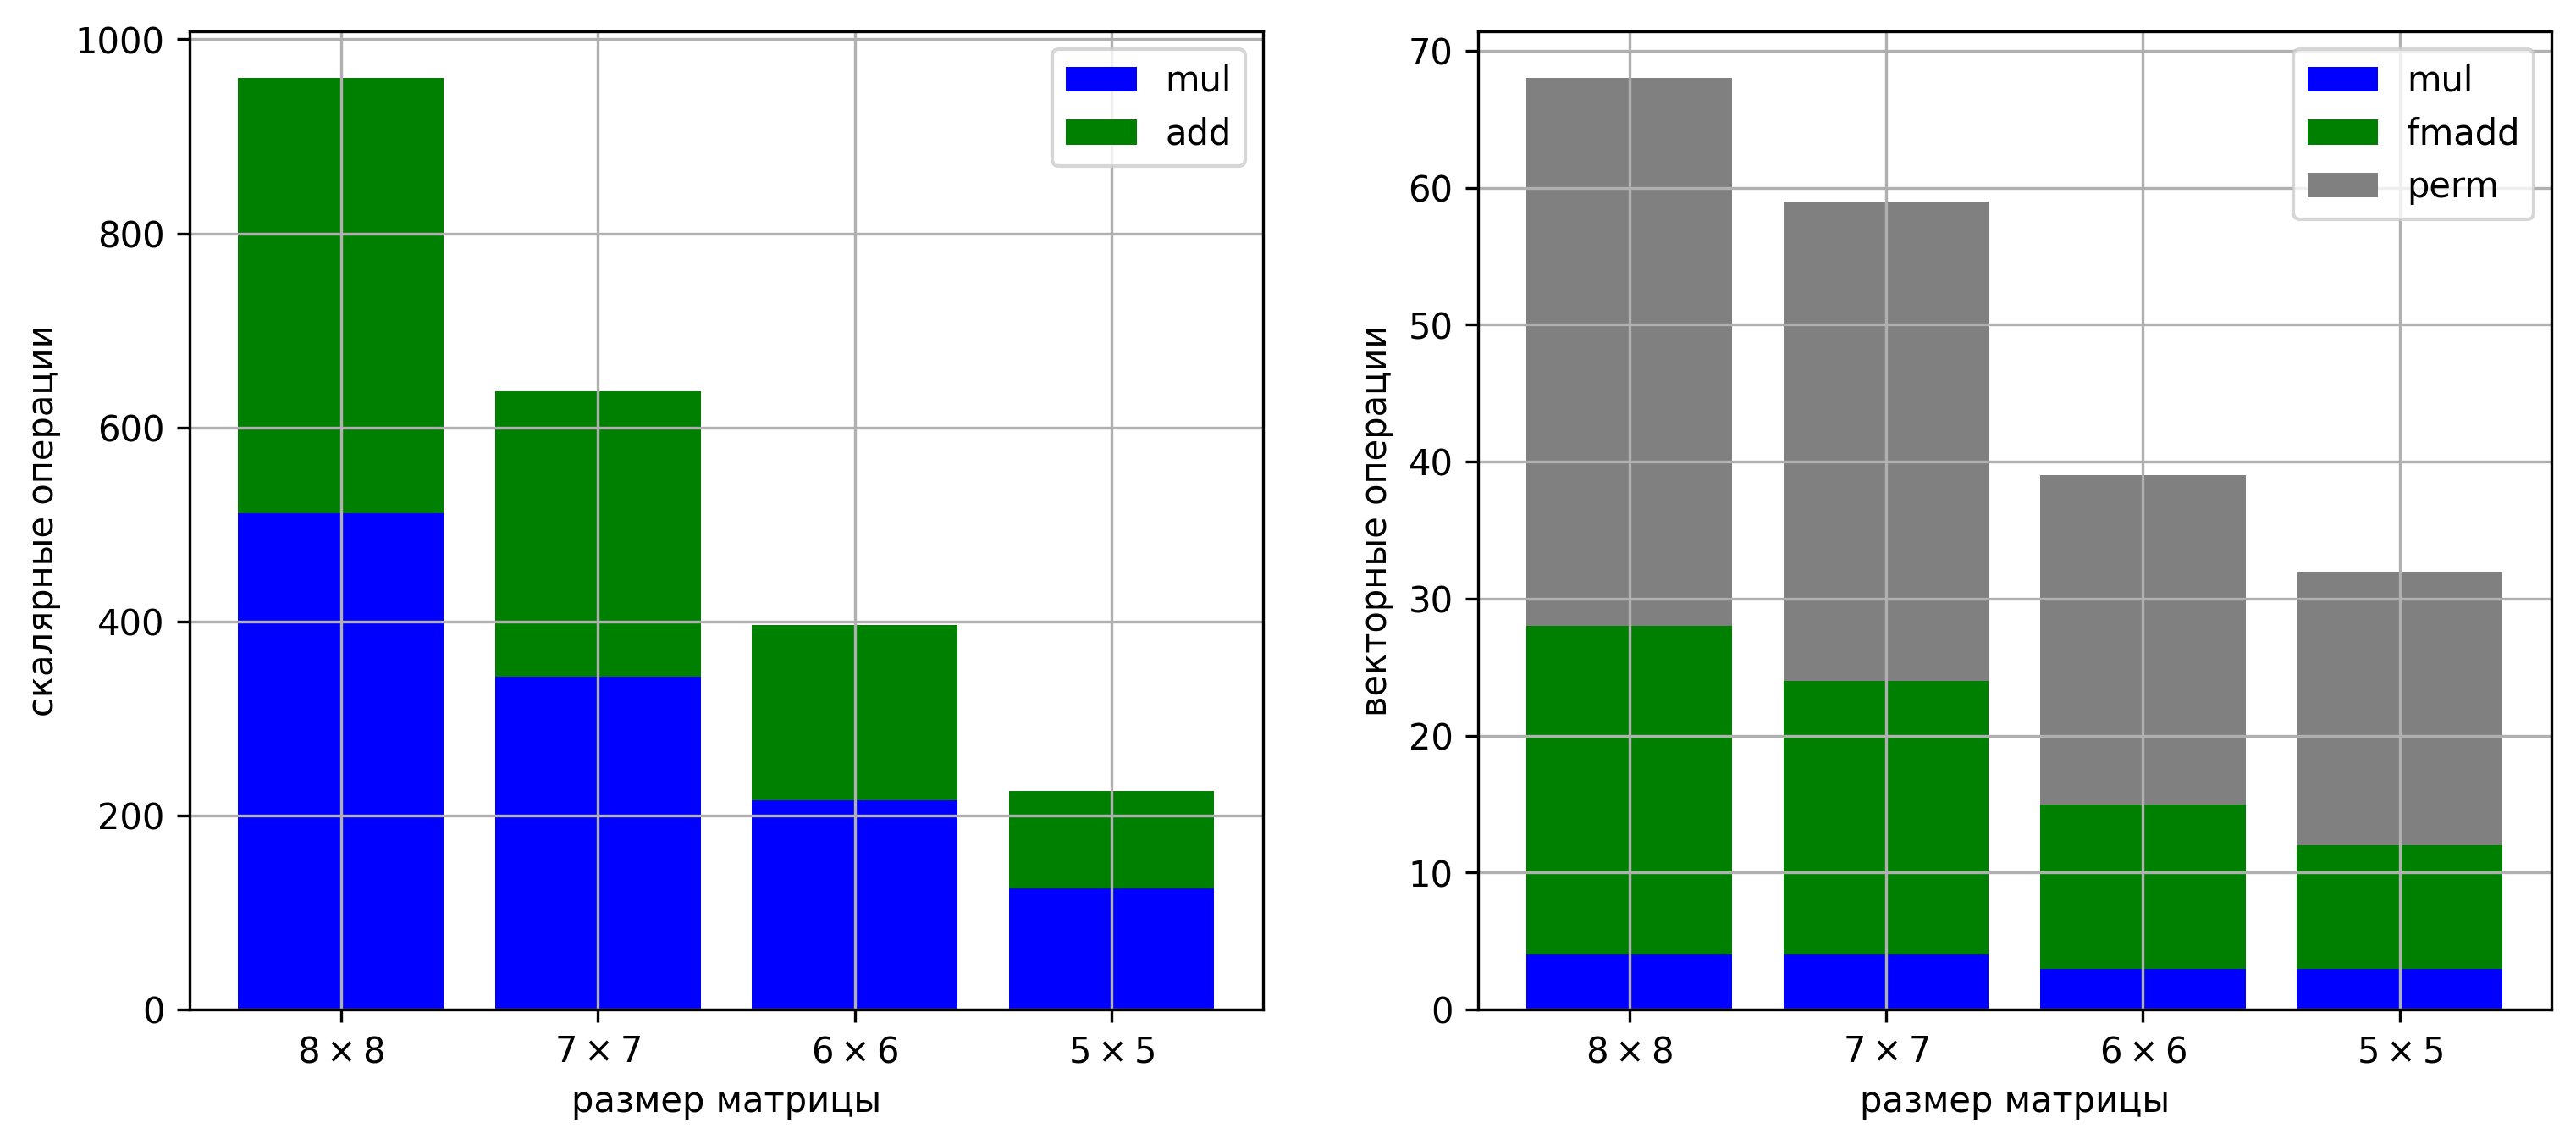
\includegraphics[width=1.00\textwidth]{./pics/text_4_spec_matr/stat.png}
\singlespacing
\captionstyle{center}\caption{Количество операций в скалярных и векторных вариантах перемножения матриц разных размеров.}
\label{fig:text_4_spec_matr_stat}
\end{figure}

На рис.~\ref{fig:text_4_spec_matr_stat} приведена статистика по количеству операций mul и add в скалярных версиях перемножения матриц, а также mul, fmadd и perm в векторизованных версиях.

\subsubsection{Замеры ускорения перемножения матриц}

Описанный способ векторизации перемножения матриц размера $8 \times 8$, $7 \times 7$, $6 \times 6$, $5 \times 5$ был опробован на процессоре Intel Xeon Phi KNL 7290\label{abbr:knl7}.
Были рассмотрены 4 функции: \texttt{mul\_8x8}, \texttt{mul\_7x7}, \texttt{mul\_6x6}, \texttt{mul\_5x5}, выполняющие перемножение матриц соответствующих размеров.
Для каждой функции были рассмотрены 3 варианта реализации.
В качестве первого варианта был использован способ векторизации с параллельным вычислением сумм элементов векторов, описанный в разделе \ref{sec:text_4_small_matr_realization} (обозначен \texttt{VECT\_OLD}), в качестве второго варианта было взято прямое ручное вычисление каждого элемента результирующей матрицы, в котором все циклы были удалены и для каждого элемента путем многократного копирования был написан скалярный код (обозначен \texttt{FULL\_UNROLL}), в качестве третьего варианта взят рассмотренный подход, основанный на обращениях только к строкам матриц и использовании комбинированных операций fmadd (обозначен \texttt{VECT\_NEW}).

\begin{figure}[ht]
\centering
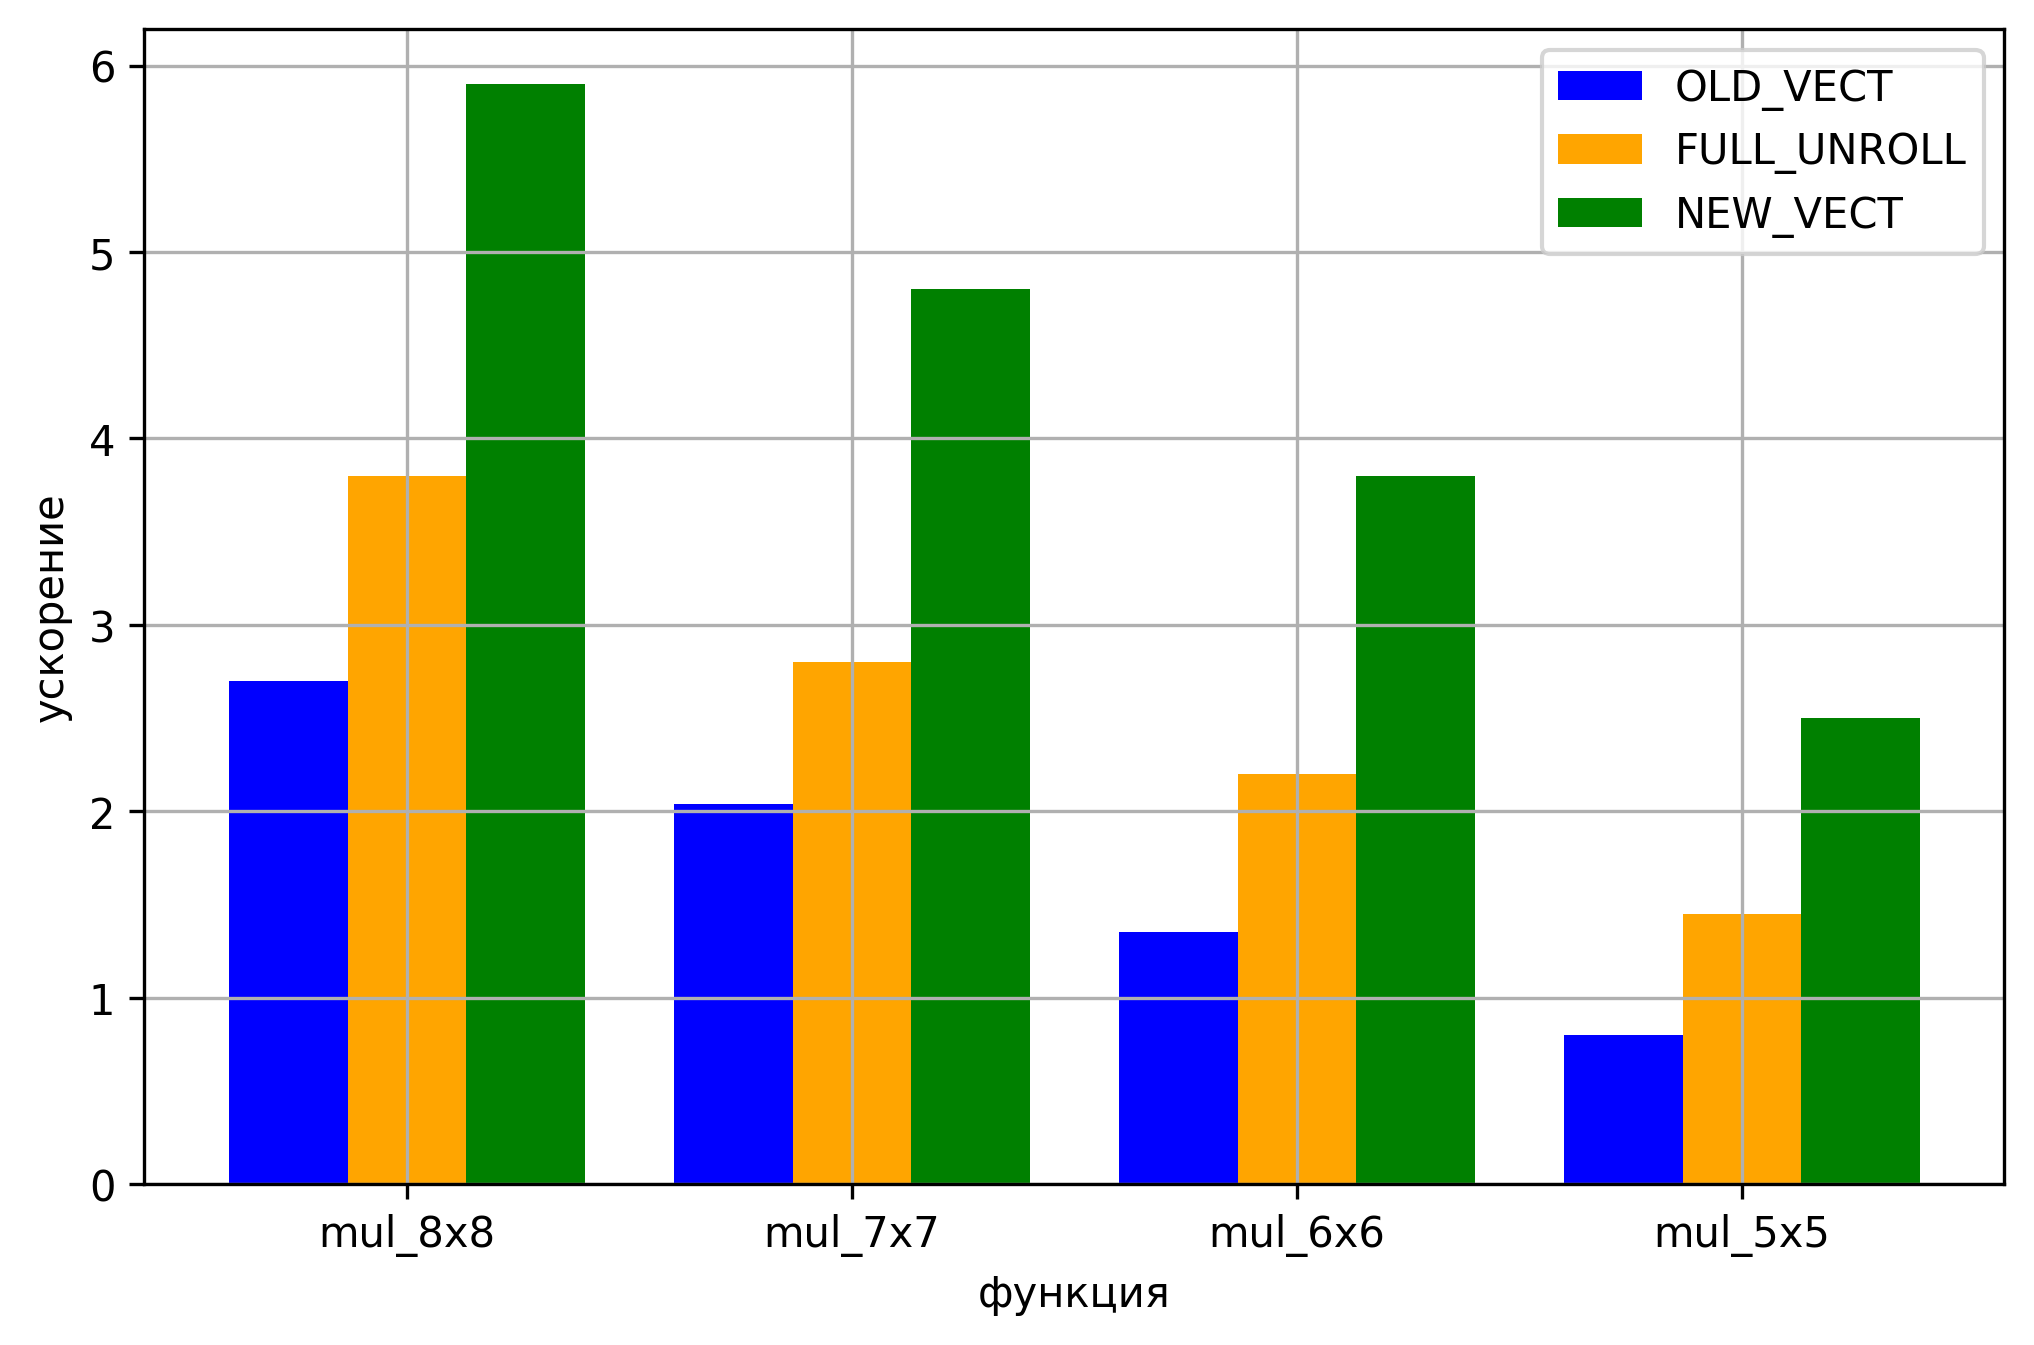
\includegraphics[width=0.6\textwidth]{./pics/text_4_spec_matr/res.png}
\singlespacing
\captionstyle{center}\caption{Ускорение и эффективность векторизации перемножения матриц с помощью подходов \texttt{OLD\_VECT}, \texttt{FULL\_UNROLL}, \texttt{NEW\_VECT}.}
\label{fig:text_4_spec_matr_res}
\end{figure}

На рис.~\ref{fig:text_4_spec_matr_res} показаны результаты тестирования описанных подходов на машине.
Из рисунка следует, что \texttt{OLD\_VECT} оказался наименее эффективным подходом, его применение даже менее выгодно, чем прямое написание скалярного кода.
Для матриц размера $5 \times 5$ этот метод оптимизации вовсе приводит к замедлению оригинальной неоптимизированной версии функции.
Метод \texttt{NEW\_VECT} демонстрирует наилучшие результаты из описанных подходов, на матрицах размера $8 \times 8$ продемонстрировано ускорение почти в 6 раз по сравнению с оригинальным кодом.
При понижении размерности матриц эффективность векторизации несколько снижается, однако даже для матриц размера $5 \times 5$ наблюдается ускорение примерно в 2,5 раза.
